\documentclass{beamer}

\usepackage{../macros}

\title{Sort}

\begin{document}

\frame{
  \titlepage
}

\begin{frame}{Popular sorting algorithm}

  \begin{block}{}
    \begin{itemize}
      \item \only<2>\emphr{Insertion sort}
      \item Selection sort
      \item Bubble sort
      \item \only<2>\emphr{Merge sort}
      \item Quicksort
    \end{itemize}
  \end{block}
\end{frame}

\begin{frame}[fragile]{Insertion sort}
  \begin{block}{Using arrays}
    \centering
    \begin{tikzpicture}[scale = 0.5]
      \draw (0, 0) rectangle (5, 1);
      \foreach \x in {1, 2, ..., 5}
        \draw (\x, 0) -- (\x, 1);
        
      \draw (0.5, 0.5) node {1};
      \draw (1.5, 0.5) node {\only<-3>{\only<2>\emphr{5}}\only<4->{\only<4>\emph{3}}};
      \draw (2.5, 0.5) node {\only<-3>{\only<3>\emphr{3}}\only<4-6>{\only<4>\emph{5}}\only<7>{\emph{4}}};
      \draw (3.5, 0.5) node {\only<-6>{\only<5>\emphr{6}}\only<7>{\emph{5}}};
      \draw (4.5, 0.5) node {\only<-6>{\only<6>\emphr{4}}\only<7>{\emph{6}}};
      
      \only<2>{\draw[rose, thick] (0, 0) rectangle (1, 1);}
      \only<3>{\draw[rose, thick] (0, 0) rectangle (2, 1);}
      \only<4-5>{\draw[rose, thick] (0, 0) rectangle (3, 1);}
      \only<6>{\draw[rose, thick] (0, 0) rectangle (4, 1);}
      \only<7>{\draw[rose, thick] (0, 0) rectangle (5, 1);}
    \end{tikzpicture}
  \end{block}
  
  \uncover<9->{
  \begin{block}{Using linked lists}
    \centering
    \begin{tikzpicture}[scale = 0.5]
%      \draw (2.5, 5) 
      \draw (0.5, 0) rectangle (1.5, 1) (0.5, 0) -- (1.5, 1) (0.5, 1) -- (1.5, 0);
      
      \uncover<-10>{\draw[->] (-1.5, 0.5) -- (0.25, 0.5);}
      
      \uncover<10->{
      \draw (0, -1.5) rectangle (2, -0.5) (1, -0.5) -- (1, -1.5);
      \draw (0.5, -1) node {3};
      \fill (1.5, -1) circle (2pt);
      }
      
      \only<11-14>{\draw[->, rounded corners] (-1.5, 0.5) -|  (-0.875, -1) -- (-0.25, -1);}
      \only<11-12>{\draw[->, rounded corners] (1.5, -1) -|  (2.5, 0.5) -- (1.75, 0.5);}
      
      \uncover<12->{
      \draw (3, -1.5) rectangle (5, -0.5) (4, -0.5) -- (4, -1.5);
      \draw (3.5, -1) node {5};
      \fill (4.5, -1) circle (2pt);
      }
      
      \uncover<13->{\draw[->, rounded corners] (4.5, -1) |- (1.75, 0.5);}
      \uncover<13-16>{\draw[->] (1.5, -1) -- (2.75, -1);}
      
      \uncover<14->{
      \draw (-0.5, -3) rectangle (1.5, -2) (0.5, -2) -- (0.5, -3);
      \draw (0, -2.5) node {1};
      \fill (1, -2.5) circle (2pt);
      }
      
      \only<15->{\draw[->, rounded corners] (-1.5, 0.5) -|  (-1.125, -2.5) -- (-0.75, -2.5);}
      \only<15->{\draw[->, rounded corners] (1, -2.5) |-  (-0.75, -1.75) |- (-0.25, -1);}
      
      \uncover<16->{
      \draw (2.5, -3) rectangle (4.5, -2) (3.5, -2) -- (3.5, -3);
      \draw (3, -2.5) node {4};
      \fill (4, -2.5) circle (2pt);
      }
      
      \only<17->{\draw[->, rounded corners=2] (1.5, -1)  -- (1.5, -1.75) --  (1.875, -1.75) -- (1.875, -2.5) -- (2.25, -2.5);}
      \only<17->{\draw[->, rounded corners] (4, -2.5) |-  (2.25, -1.75) |- (2.75, -1);}
      
      
    \end{tikzpicture}
  \end{block}}
\end{frame}

\begin{frame}{Merge sort}

  \begin{block}{Dichotomic sort}
    \centering
    \begin{tikzpicture}[scale = 0.45]
      \draw (0, 0) rectangle (5, 1);
      \foreach \x in {1, 2, ..., 5}
        \draw (\x, 0) -- (\x, 1);
        
      \draw (0.5, 0.5) node {1};
      \draw (1.5, 0.5) node {5};
      \draw (2.5, 0.5) node {3};
      \draw (3.5, 0.5) node {6};
      \draw (4.5, 0.5) node {4};
      
      \only<2->{\draw[rose, thick] (2, 1) -- (2, 0);}
      
      \uncover<3->{
      \draw[rose, ->] (1, -0.2) -- (0, -0.8);
      \draw[rose, ->] (3.5, -0.2) -- (4.5, -0.8);
      
      \draw (-1, -2) rectangle (1, -1);
      \draw (3, -2) rectangle (6, -1);
      \foreach \x in {0, 4, 5}
        \draw (\x, -2) -- (\x, -1);
        
      \draw (-0.5, -1.5) node {1};
      \draw (0.5, -1.5) node {5};
      \draw (3.5, -1.5) node {3};
      \draw (4.5, -1.5) node {6};
      \draw (5.5, -1.5) node {4};
      }
      
      \only<4->{\draw[rose, thick] (0, -1) -- (0, -2);}
      
      \uncover<5->{
      \draw[rose, ->] (-0.5, -2.2) -- (-1, -2.8);
      \draw[rose, ->] (0.5, -2.2) -- (1, -2.8);
      
      \draw (-1.5, -4) rectangle (-0.5, -3);
      \draw (0.5, -4) rectangle (1.5, -3);
      
      \draw (-1, -3.5) node {1};
      \draw (1, -3.5) node {5};
      }
      
      \uncover<6->{
      \draw[vert, <-] (-0.5, -4.8) -- (-1, -4.2);
      \draw[vert, <-] (0.5, -4.8) -- (1, -4.2);
      \draw (-1, -6) rectangle (1, -5) (0, -6) -- (0, -5);
      \draw (-0.5, -5.5) node {1};
      \draw (0.5, -5.5) node {5};
      }
      
      \only<7->{\draw[rose, thick] (4, -1) -- (4, -2);}
      \uncover<8->{
      \draw[rose, ->] (3.5, -2.2) -- (3, -2.8);
      \draw[rose, ->] (5, -2.2) -- (5.5, -2.8);
      
      \draw (2.5, -4) rectangle (3.5, -3);
      \draw (4.5, -4) rectangle (6.5, -3) (5.5, -4) -- (5.5, -3);
      
      \draw (3, -3.5) node {3};
      \draw (5, -3.5) node {6};
      \draw (6, -3.5) node {4};
      }
      
      \only<9->{\draw[rose, thick] (5.5, -4) -- (5.5, -3);}
      \uncover<10->{
      \draw[rose, ->] (5, -4.2) -- (4.5, -4.8);
      \draw[rose, ->] (6, -4.2) -- (6.5, -4.8);

      \draw (4, -6) rectangle (5, -5);
      \draw (6, -6) rectangle (7, -5);
      
      \draw (4.5, -5.5) node {6};
      \draw (6.5, -5.5) node {4};
      }
      
      \uncover<11->{
      \draw[vert, <-] (5, -6.8) -- (4.5, -6.2);
      \draw[vert, <-] (6, -6.8) -- (6.5, -6.2);
      \draw (4.5, -8) rectangle (6.5, -7) (5.5, -8) -- (5.5, -7);
      \draw (6, -7.5) node {6};
      \draw (5, -7.5) node {4};
      }
      
      \uncover<12->{
      \draw[vert, <-] (3.5, -8.8) -- (3, -4.2);
      \draw[vert, <-] (5, -8.8) -- (5.5, -8.2);
      
      \draw (3, -10) rectangle (6, -9) (4, -10) -- (4, -9) (5, -10) -- (5, -9);
        
      \draw (3.5, -9.5) node {3};
      \draw (4.5, -9.5) node {4};
      \draw (5.5, -9.5) node {6};
      }
      
      \uncover<13->{
      \draw[vert, <-] (1, -10.8) -- (0, -6.2);
      \draw[vert, <-] (3.5, -10.8) -- (4.5, -10.2);
      
      \draw (0, -12) rectangle (5, -11);
      \foreach \x in {1, 2, ..., 5}
        \draw (\x, -12) -- (\x, -11);
        
      \draw (0.5, -11.5) node {1};
      \draw (1.5, -11.5) node {3};
      \draw (2.5, -11.5) node {4};
      \draw (3.5, -11.5) node {5};
      \draw (4.5, -11.5) node {6};
      }
      
    \end{tikzpicture}
  \end{block}
\end{frame}

\begin{frame}{Exercise 1: Candy Distribution}
  Using two lists with insertion sort
  
  Using the sort procedure in your preferred language
  
\end{frame}

\begin{frame}{Exercise 2: Inversion Count}
  Using Merge sort
  
\end{frame}

\begin{frame}{Exercise 3: It's a Murder}
  Using Merge sort
  
\end{frame}

\end{document}
